\documentclass{article}
\usepackage[utf8]{inputenc}
\usepackage{graphicx}
\graphicspath{ {./images/} }

\title{TDT4173  - Task 1}
\author{Håvard Hjelmeseth}
\date{September 2021}

\begin{document}

\maketitle

\section{K-means algorithm}
For my first algorithm i have decided to implement the K-means algorithm
, which is an unsupervised learning algorithm for data classification.

\subsection{First dataset}
The first dataset contains points in a 2D space, where the points seem to have
a natural separation into two clusters. The implementation of the algorithm
seems to have no issues with this dataset.

\begin{figure}[!h]
    \centering
    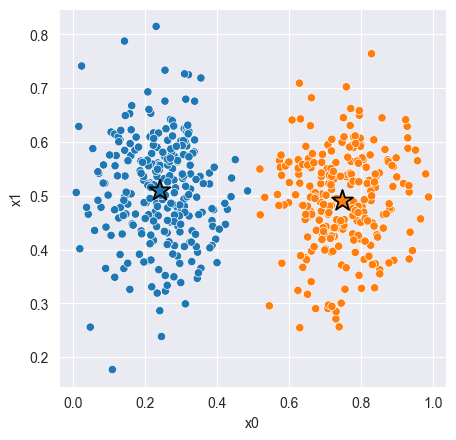
\includegraphics[width=0.75\textwidth]{kmeans_data1.png}
    \caption{First dataset classification with k-means}
    \label{fig:dataset1}
\end{figure}

\subsection{Second dataset}

The second dataset is a bit harder, where the points are still in a 2D space,
but does not longer have a natural separation into two clusters. Running the kmeans
algorithm with k=10 clusters seems to give a good result as seen in the plots.

\begin{figure}[h]
    \centering
    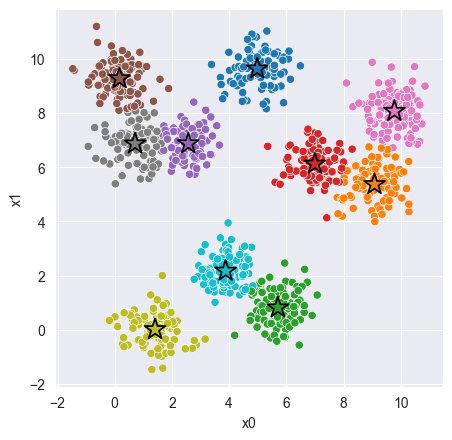
\includegraphics[width=0.75\textwidth]{kmeans_data2.png}
    \caption{Second dataset classification with k-means}
    \label{fig:dataset2}
\end{figure}


\section{Second algorithm}

\end{document}
